\documentclass{article}

\usepackage{graphicx}
\usepackage{authblk}
\usepackage{listings}
\usepackage{xcolor}
\usepackage[a4paper,
            bindingoffset=0.2in,
            left=0.5in,
            right=0.5in,
            top=0.5in,
            bottom=0.5in,
            footskip=.25in]{geometry}

\definecolor{mGreen}{rgb}{0,0.6,0}
\definecolor{mGray}{rgb}{0.5,0.5,0.5}
\definecolor{mPurple}{rgb}{0.58,0,0.82}
\definecolor{backgroundColour}{rgb}{0.95,0.95,0.92}

\lstdefinestyle{CStyle}{
    backgroundcolor=\color{backgroundColour},   
    commentstyle=\color{mGreen},
    keywordstyle=\color{magenta},
    numberstyle=\tiny\color{mGray},
    stringstyle=\color{mPurple},
    basicstyle=\footnotesize,
    breakatwhitespace=false,         
    breaklines=true,                 
    captionpos=b,                    
    keepspaces=true,                 
    numbers=left,                    
    numbersep=5pt,                  
    showspaces=false,                
    showstringspaces=false,
    showtabs=false,                  
    tabsize=2,
    language=C
}


\title{Lab Exercise 4: Using the DE10-Lite \& Repetition and Selection}
\author{Cody Raposa}
\affil{ELEC2850 Microcontrollers Using C Programming}

\begin{document}
\maketitle
\begin{flushleft}
  \section{Problem Statement}
  Create a program that will find the real roots of a quadratic equation. The program should prompt the user to enter the values of a, b, and c. The program should then calculate the roots of the equation using the quadratic formula, then displaying the roots.
  %\section{Assumptions}
  %\section{Algorithm}
  \section{Analysis}
  \subsection{Inputs}
  num1, num2, num3 (int)
  \subsection{Outputs}
  rootOne, rootTwo (floats)
  \subsection{Formulas}
  Quadratic Formula: $x = \frac{-b \pm \sqrt{b^2 - 4ac}}{2a}$
  %\section{Pseudocode}
  \section{Flowchart}
    \begin{figure}[!h]
      \begin{centering}
        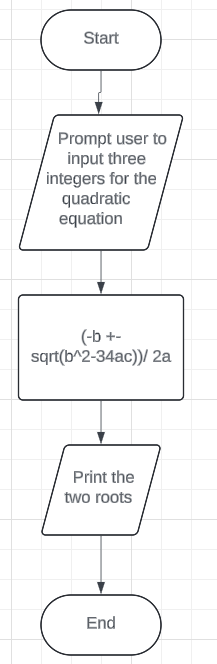
\includegraphics[scale=0.5]{Q1.png}
        \caption{Flowchart for finding the roots of a quadratic equation}
      \end{centering}
    \end{figure}
    \newpage
  \section{Output}
  \begin{figure}[!h]
    \begin{centering}
      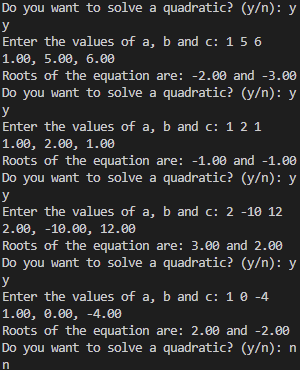
\includegraphics[scale=1]{P3_t1.png}
      \caption{Four test cases for the program}
    \end{centering}
  \end{figure}
  \section{Code}
  \lstinputlisting[style=CStyle]{P3.c}
\newpage
\section{Part 4}
\begin{figure}[!h]
    \begin{centering}
        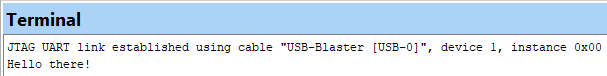
\includegraphics[scale=0.5]{Test_Terminal.png}
        \caption{Hello World runnning on the DE10}
    \end{centering}
\end{figure}
\begin{figure}[!h]
    \begin{centering}
        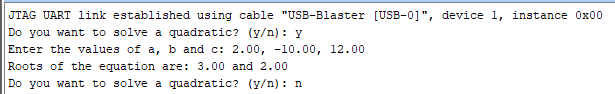
\includegraphics[scale=0.5]{P4_output.png}
        \caption{Part 3 code runnning on the DE10}
    \end{centering}
\end{figure}
\end{flushleft}
\end{document}